% !TEX TS-program = XeLaTeX
% use the following command:
% all document files must be coded in UTF-8
\documentclass[spanish]{textolivre}
% build HTML with: make4ht -e build.lua -c textolivre.cfg -x -u article "fn-in,svg,pic-align"

\journalname{Texto Livre}
\thevolume{16}
%\thenumber{1} % old template
\theyear{2023}
\receiveddate{\DTMdisplaydate{2022}{11}{15}{-1}} % YYYY MM DD
\accepteddate{\DTMdisplaydate{2022}{12}{20}{-1}}
\publisheddate{\DTMdisplaydate{2023}{1}{2}{-1}}
\corrauthor{Daniel Cassany}
\articledoi{10.1590/1983-3652.2023.41797}
%\articleid{NNNN} % if the article ID is not the last 5 numbers of its DOI, provide it using \articleid{} commmand 
% list of available sesscions in the journal: articles, dossier, reports, essays, reviews, interviews, editorial
\articlesessionname{dossier}
\runningauthor{Allué y Cassany} 
%\editorname{Leonardo Araújo} % old template
\sectioneditorname{Hugo Heredia Ponce}
\layouteditorname{Daniervelin Pereira}

\title{Grabando vídeos: educación literaria multimodal}
\othertitle{Gravando vídeos: educação literária multimodal}
\othertitle{Video recording: literate multimodal education}
% if there is a third language title, add here:
%\othertitle{Artikelvorlage zur Einreichung beim Texto Livre Journal}

\author[1]{Consuelo Allué~\orcid{0000-0002-3113-3362}\thanks{Email: \href{mailto:mconsolacion.allue@unavarra.es}{mconsolacion.allue@unavarra.es}}}
\author[2]{Daniel Cassany~\orcid{0000-0003-3494-5531}\thanks{Email: \href{mailto:daniel.cassany@upf.edu}{daniel.cassany@upf.edu}}}
\affil[1]{Universidad Pública de Navarra, Facultad de Ciencias Humanas, Sociales y de la Educación, Departamento de Ciencias Humanas y de la Educación, Pamplona, España.}
\affil[2]{Universitat Pompeu Fabra, Facultad de Traducció i Ciències del Llenguatge, Departament de Traducció i Ciències del Llenguatge, Barcelona, España.}

\addbibresource{article.bib}
% use biber instead of bibtex
% $ biber article

% used to create dummy text for the template file
\definecolor{dark-gray}{gray}{0.35} % color used to display dummy texts
\usepackage{lipsum}
\SetLipsumParListSurrounders{\colorlet{oldcolor}{.}\color{dark-gray}}{\color{oldcolor}}

% used here only to provide the XeLaTeX and BibTeX logos
\usepackage{hologo}

% if you use multirows in a table, include the multirow package
\usepackage{multirow}

% provides sidewaysfigure environment
\usepackage{rotating}

% CUSTOM EPIGRAPH - BEGIN 
%%% https://tex.stackexchange.com/questions/193178/specific-epigraph-style
\usepackage{epigraph}
\renewcommand\textflush{flushright}
\makeatletter
\newlength\epitextskip
\pretocmd{\@epitext}{\em}{}{}
\apptocmd{\@epitext}{\em}{}{}
\patchcmd{\epigraph}{\@epitext{#1}\\}{\@epitext{#1}\\[\epitextskip]}{}{}
\makeatother
\setlength\epigraphrule{0pt}
\setlength\epitextskip{0.5ex}
\setlength\epigraphwidth{.7\textwidth}
% CUSTOM EPIGRAPH - END

% LANGUAGE - BEGIN
% ARABIC
% for languages that use special fonts, you must provide the typeface that will be used
% \setotherlanguage{arabic}
% \newfontfamily\arabicfont[Script=Arabic]{Amiri}
% \newfontfamily\arabicfontsf[Script=Arabic]{Amiri}
% \newfontfamily\arabicfonttt[Script=Arabic]{Amiri}
%
% in the article, to add arabic text use: \textlang{arabic}{ ... }
%
% RUSSIAN
% for russian text we also need to define fonts with support for Cyrillic script
% \usepackage{fontspec}
% \setotherlanguage{russian}
% \newfontfamily\cyrillicfont{Times New Roman}
% \newfontfamily\cyrillicfontsf{Times New Roman}[Script=Cyrillic]
% \newfontfamily\cyrillicfonttt{Times New Roman}[Script=Cyrillic]
%
% in the text use \begin{russian} ... \end{russian}
% LANGUAGE - END

% EMOJIS - BEGIN
% to use emoticons in your manuscript
% https://stackoverflow.com/questions/190145/how-to-insert-emoticons-in-latex/57076064
% using font Symbola, which has full support
% the font may be downloaded at:
% https://dn-works.com/ufas/
% add to preamble:
% \newfontfamily\Symbola{Symbola}
% in the text use:
% {\Symbola }
% EMOJIS - END

% LABEL REFERENCE TO DESCRIPTIVE LIST - BEGIN
% reference itens in a descriptive list using their labels instead of numbers
% insert the code below in the preambule:
%\makeatletter
%\let\orgdescriptionlabel\descriptionlabel
%\renewcommand*{\descriptionlabel}[1]{%
%  \let\orglabel\label
%  \let\label\@gobble
%  \phantomsection
%  \edef\@currentlabel{#1\unskip}%
%  \let\label\orglabel
%  \orgdescriptionlabel{#1}%
%}
%\makeatother
%
% in your document, use as illustraded here:
%\begin{description}
%  \item[first\label{itm1}] this is only an example;
%  % ...  add more items
%\end{description}
% LABEL REFERENCE TO DESCRIPTIVE LIST - END


% add line numbers for submission
%\usepackage{lineno}
%\linenumbers

\begin{document}
\maketitle

\begin{polyabstract}
\begin{abstract}
El uso del vídeo en la educación literaria va ganando terreno en el aula con la diseminación tecnológica y de redes sociales. Más allá de la visualización de adaptaciones cinematográficas, docentes y alumnos empiezan a producir vídeos propios con objetivos de educación literaria y lingüística. En este contexto, nos preguntamos cómo se desarrolla esta práctica en la educación secundaria, con qué características (géneros, temas, estilos, audiencias) y metodologías (objetivos, evaluación, andamiajes, interacción) y con qué grado de satisfacción. A partir del análisis de contenido de 102 vídeos discentes y de 11 entrevistas semiestructuradas a docentes experimentados, concluimos que es una práctica emergente, diversa y motivadora, centrada en el desarrollo de la competencia literaria y lingüística, que sitúa al aprendiz en el centro de la clase, fomenta el aprendizaje cooperativo y facilita la apropiación personal de contenidos curriculares. Se producen vídeos breves, técnicamente variados, que exigen destrezas orales y escritas específicas, receptivas y productivas, que manejan contenidos literarios diversos, según la aproximación más historicista o competencial de la educación literaria.

\keywords{Vídeo discente \sep Literatura multimodal \sep Agencia del aprendiz \sep Booktuber}
\end{abstract}

\begin{portuguese}
\begin{abstract}
O uso do vídeo na educação literária vem ganhando espaço na sala de aula com a disseminação da tecnologia e das redes sociais. Além de assistir a adaptações cinematográficas, professores e alunos começam a produzir seus próprios vídeos para fins de educação literária e linguística. Nesse contexto, questionamo-nos como se desenvolve essa prática no ensino secundário, com que caraterísticas (gêneros, temáticas, estilos, públicos) e metodologias (objetivos, avaliação, andaime, interação) e com que grau de satisfação. Com base na análise de conteúdo de 102 vídeos de alunos e 11 entrevistas semiestruturadas com professores experientes, concluímos que é uma prática emergente, diversificada e motivadora, focada no desenvolvimento da competência literária e linguística, que coloca o aluno no centro da da turma, estimula a aprendizagem cooperativa e facilita a apropriação pessoal dos conteúdos curriculares. São produzidos vídeos curtos e tecnicamente variados, que exigem habilidades orais e escritas específicas, receptivas e produtivas, que manuseiam conteúdos literários diversos, segundo a abordagem mais historicista ou de competência da educação literária.

\keywords{Vídeo do aluno \sep Literatura multimodal \sep Agência do aluno \sep Booktuber}
\end{abstract}
\end{portuguese}

\begin{english}
\begin{abstract}
The use of video in literary education is gaining spaces in the classroom, with the dissemination of technology and social networks. Beyond the visualization of film adaptations, teachers and learners are beginning to produce personal videos for literary and linguistic education purposes. In this context, we try to understand how this practice is developed in secondary education, with which characteristics (genres, themes, styles, audiences) and methodologies (objectives, evaluation, scaffolding, interaction) and with which degree of satisfaction. Based on content analysis of 102 student videos and 11 semi-structured interviews with experienced teachers, we conclude that it is an emerging, diverse and motivating practice, focused on the development of literary and linguistic competence, which places the learner at the center of the classroom, encourages cooperative learning and facilitates personal appropriation of curricular content. Short and technically varied videos are produced with specific oral and written skills, receptive and productive, that manage very diverse literary content, depending on the most historicist or competency-based approach of the literary education.

\keywords{Learner video \sep Multimodal literature \sep Learner agency \sep Booktuber}
\end{abstract}
\end{english}
% if there is another abstract, insert it here using the same scheme
\end{polyabstract}

\section{Introducción}\label{sec-intro}
La literatura y su enseñanza y aprendizaje no quedan al margen de la revolución digital, sin duda, y poco a poco experimentan mutaciones diversas según avanza la digitalización (programa 1x1, tabletas). Aunque muchas escuelas se mantengan adheridas al libro escrito y a las interpretaciones canónicas, la práctica literaria abandona poco a poco el grafocentrismo para ganar multimodalidad y multimedialidad, y transgrede el circuito analógico (autor-editorial-librería/biblioteca-lector) para explorar nuevos canales de interacción entre autor y lectores \cite{milyakina_rethinking_2018}. Más allá de si leemos con ebook, si la juventud lee menos o si los adultos sustituimos la prescripción de autoridad (revistas, críticas, bibliotecas) por las redes sociales (Goodreads, Amazon), educar la competencia literaria con jóvenes que llevan un móvil en el bolsillo, gestionan varios perfiles en la red y siguen sus series favoritas por \textit{streaming}, no puede basarse en las prácticas letradas ancestrales y constituye un reto mayúsculo.

Por ello, parte de la investigación actual en didáctica se centra en las prácticas digitales desarrolladas con literatura, dentro y fuera del aula, que generan enseñanza-aprendizaje, como el reciente diagnóstico sobre la lectura \cite{cruces_villalobos_como_2017} o el monográfico de Ocnos sobre “Prácticas Literarias Digitales” \cite{cassany_editorial:_2021}, con trabajos sobre tertulias y clubes de lectura en línea, fandom, redes sociales o videojuegos. En este contexto los campos en que ha habido más investigación son, sin ánimo de exhaustividad, la \textit{fanfiction} \cite{black_adolescents_2008}, los \textit{booktubers} \cite{rovira-collado_booktrailer_2017} y el \textit{booktrailer} \cite{tabernero_sala_book_2013} o los videojuegos \cite{ramada_prieto_esto_2017}, y no es casualidad que los tres últimos ejemplos tengan el vídeo como formato comunicativo.

Poco a poco el vídeo está adquiriendo más protagonismo en la vida cotidiana, la producción cultural y también la educación, con la proliferación de móviles y redes sociales. Para muchos estudiantes ya es su formato básico de comunicación (Instagram, TikTok, YouTube, Netflix) y cada vez más docentes lo introducen. También en la investigación surgen espacios específicos como el \hyperlink{https://brill.com/view/journals/vjep/vjep-overview.xml}{Video Journal of Education and Pedagogy}. Nuestro proyecto ForVid (ver Sección \ref{sec-conclusao}) se sitúa en este marco para describir y analizar las prácticas videográficas que fomentan aprendizaje lingüístico, tanto dentro del aula \cite{cassany_editorial:_2021} como fuera, en contextos de ocio \cite{cassany_daniel_coord._fandom_2019}. En este trabajo nos centramos en el uso del vídeo que hacen los docentes de literatura (o lengua y literatura) en la educación secundaria.

\section{Vídeos en la educación literaria}\label{sec-normas}
Trazamos un sucinto panorama de la investigación sobre el vídeo en la educación literaria dentro del ámbito de la didáctica de la lengua y la literatura. Por ello descartamos los trabajos de otros campos (cine, periodismo, teatro, tecnología) que pueden ser afines a nuestro campo, pero que adoptan otras perspectivas.

Partimos de una exploración bibliográfica previa \cite{cassany_ya_2021} que, entre otros aspectos, identificó tres grandes modalidades de uso del vídeo para la educación: la visualización de vídeos, la producción de vídeos discentes y la producción de vídeos docentes. Esta exploración mostró también que la investigación previa se ha volcado en la primera modalidad (contenidos curriculares del vídeo, diseño de vídeos educativos, interacción en clase con vídeos, YouTube en el aula) y que el conjunto valora positivamente esta práctica por su motivación.

En cambio, la investigación previa sobre la segunda modalidad (vídeos discentes), que es la que interesa aquí, ofrece menos resultados y suele tratarse de estudios de caso que describen prácticas innovadoras de producción de vídeos en las materias de idioma, alfabetización mediática, participación cívica y trabajo cooperativo. Estos trabajos concluyen que la grabación de vídeos es versátil y ofrece beneficios para propósitos tanto disciplinarios (idiomas, sociales) como interdisciplinarios (alfabetización mediática, aprendizaje cooperativo, creatividad). Pero muchos de estos estudios \cite{hobbs_past_2009} analizan proyectos interdisciplinarios de grabación de vídeos, con varias materias y mucho tiempo de aula, que inevitablemente se alejan de nuestro campo, restringido al aula de Literatura o Lengua y Literatura.

En el ámbito de la educación literaria, la visualización de películas llega a las aulas a partir de los años ochenta \cite{ferres_video_1992}. Se utilizaba con fines motivacionales para fomentar la lectura de clásicos después de visualizar sus adaptaciones cinematográficas, o para contextualizar la época histórica en que surgió una obra, autor o movimiento (juglares, trovadores). En idioma extranjero, el interés por la visualización de vídeos en lengua meta fortalece la comprensión oral, tradicionalmente abandonada, que había empezado a incrementar su protagonismo gracias a la grabación oral. Sin duda, la inclusión de imágenes en movimiento dota a esta tarea receptiva de más contexto sociocultural y permite entender mejor las interacciones y los contextos comunicativos. En este marco, el uso del vídeo en el aula pasó a ser una cuestión básica de la formación del profesorado de idioma.

La producción de vídeos amateurs es más reciente, estimulada por la expansión tecnológica y las redes sociales videográficas (YouTube en 2005; Instagram Stories en 2016; TikTok en 2016). En 2009 el segundo coautor descubrió en YouTube una docena de vídeos de estudiantes de magisterio mexicanos que reseñaban obras suyas a modo de tarea final de evaluación. También en 2009 surge la primera booktuber angloparlante, como un subtipo de \textit{youtuber} o \textit{influencer} joven de la literatura juvenil, con decenas de miles de seguidores, mientras que los primeros \textit{booktubers} hispanos nacen pocos años después (Javier Ruescas en 2010; Fa Orozco en 2012, según Wikipedia en español).

Otro videogénero coetáneo es el \textit{booktrailer} (\textit{bibliotráiler o tráiler de libro}), documentado en YouTube en 2006 como la adaptación para el libro de la popular técnica de márquetin de avanzar el estreno de una película con un anuncio breve. Al respecto, la Wikipedia catalana afirma que esta transferencia transmedia causó furor en la época, al aprovechar recursos cinematográficos para presentar libros y que hoy se utiliza para “promocionar libros desde una editorial, trabajar la literatura en clase o introducir la literatura entre la generación digital”, con secciones de “cómo hacerlo” o “qué características debe tener”.

Según las bases bibliográficas, estos dos videogéneros literarios han despertado el interés de muchos investigadores latinoamericanos en los últimos 5 años, con más de un centenar de trabajos para cada uno, entre tesis doctorales \cite{tomasena_glennie_booktubers_2020,paladines_literacy_2022}, análisis de prácticas comunicativas y aprendizaje informal \cite{vizcaino-verdu_reading_2019}, aplicaciones para la formación docente \cite{ibarra_rius_book_2016,heredia-ponce_booktrailer_2020} o exploraciones en varias redes sociales \cite{quiles_cabrera_textos_2020} y países (Argentina: \cite{albarello_booktubers_2019}; Brasil: \cite{fialho_booktubers_2023}), con una mayoría de estudios sobre jóvenes y algunos sobre niños \cite{lopez-gil_promocion_2021}. 

En concreto, los estudios citados sobre booktubers españoles y brasileños coinciden en varios aspectos: 1) la mayoría de autores son mujeres blancas jóvenes; 2) sus vídeos reciben millones de visualizaciones y decenas de miles de seguidores; 3) la respuesta de la audiencia consiste en dar \textit{I like} al vídeo y escribir comentarios que merecen réplicas del autor u otros seguidores; 4) se presentan y comentan diversidad de géneros literarios; 5) esta práctica transforma YouTube “em um atrativo cenário de aprendizagem e de incentivo à leitura” \cite{fialho_booktubers_2023}, y 6) se transgreden así los límites de la educación literaria tradicional, de la prescripción académica o del grafocentrismo.

La búsqueda bibliográfica sobre otros géneros videográficos literarios aporta resultados interesantes sobre todo con la narración digital y la videopoesía. Respecto a la primera, más conocida en su denominación inglesa \textit{digital storytelling} (DST), el vídeo constituye uno de los formatos más frecuentes para elaborar estos relatos digitales interactivos, autobiográficos o inventados, que integran diversidad de lenguajes y que se han popularizado desde principios de siglo tanto en la educación como en otros campos (salud, publicidad, entretenimiento) \cite{godwin-jones_digital_2012}. El completo metaanálisis de \textcite{quah_systematic_2022} confirma su interés para primaria y secundaria con la mejora de la alfabetización, la creatividad o la formación tecnológica. También la experiencia con escuelas rurales multinivel asturianas de \textcite{del_moral_perez_competencias_2017} destaca las mejoras en expresión, coherencia del relato y nociones espacio-temporales del alumnado que aporta esta práctica.

Respecto a la videopoesía, hallamos numerosos estudios de caso y propuestas didácticas en los repositorios digitales para docentes (TFM, recursos, etc.) que utilizan la grabación de poemas para desarrollar la competencia literaria o incrementar las destrezas orales. En esta línea, \textcite{de_la_torre_literatura_2022} recopila un corpus de poesía digital (videopoesía, poesía spam, poesía visual y poesía y código) con propuestas didácticas para la enseñanza de español como lengua extranjera, y \textcite{hoglund_video_2017} analiza con detalle como los adolescentes de secundaria aprovechan los recursos multimodales de la grabación de vídeos para construir y negociar su interpretación personal de la poesía.

Respecto a otro género emergente como el videojuego, en su metaanálisis centrado en secundaria, \textcite{rojas-garcia_alisis_2022} hallan 19 investigaciones desde 2016, que indican una mayor presencia de este género en Europa que en Latinoamérica, con buenos resultados educativos en aspectos cognitivos y socioemocionales, pero con una mayoría de propuestas centradas en las matemáticas y con escasa presencia de las humanidades. Finalmente, un estudio sobre la utilización de las tecnologías digitales (incluido el vídeo) en secundaria \cite{rodriguez_munoz_competencia_2021} muestra que los docentes obtienen resultados útiles sobre “elementos narratológicos y animación a la lectura”; también revela que los docentes jóvenes muestran más interés por este recurso, mientras que los maduros se adhieren a formatos más tradicionales.

En resumen, constatamos la existencia de algunas investigaciones revelantes sobre algunos videogéneros literarios particulares (\textit{booktubers}, \textit{booktrailers}, narración digital, videopoesía), pero no hallamos trabajos que exploren de manera más global el aprovechamiento de la grabación en vídeo de aprendices para la educación literaria multimodal. Con este trabajo, dentro del proyecto mencionado ForVid, esperamos poder aportar luz sobre este nicho.

\section{Preguntas de investigación}\label{sec-conduta}
En este contexto, nuestras preguntas de investigación son:

\begin{enumerate}
    \item ¿Qué tipo de vídeos produce el alumnado y qué aprendizajes lingüísticos y literarios facilitan?
    \item ¿Qué potencialidades y limitaciones presenta la grabación de vídeos de estudiantes en secundaria en las materias de lenguas y literatura?
\end{enumerate}

La primera pregunta propone describir el contenido (géneros, temas, enfoque, estilo) y la forma (duración, modos, actividad lingüística) para identificar su rentabilidad. La segunda aborda de manera más operativa las ventajas y los inconvenientes que presenta en el contexto educativo de secundaria en España para poder ofrecer recomendaciones y orientaciones al docente.


\section{Metodología y corpus}\label{sec-fmt-manuscrito}
Reclutamos intencionalmente a docentes en activo que proponen grabar vídeos a sus alumnos en nuestro entorno inmediato, entre centros colaboradores, colegas o conocidos de colegas. Esta estrategia de bola de nieve permitió contactar con 25 docentes, de los que elegimos 11 por estos criterios de inclusión: 1) trabajar en centros de secundaria públicos o concertados; 2) dar clases de las lenguas (castellano, eusquera, catalán, inglés) y sus literaturas; 3) proponer de manera continuada al alumnado tareas de grabación de vídeos; 4) aportar al proyecto ejemplos propios de estos vídeos, los materiales relacionados y una entrevista, y 4) aceptar los requerimientos éticos habituales de investigación. Descartamos algunos candidatos muy activos por incumplir alguno de estos criterios. La \Cref{tab01} resume nuestros datos:

\begin{table}[h!]
\begin{threeparttable}
\caption{Datos del corpus.}
\label{tab01}
\centering \small
\begin{tabular}{p{2.5cm} >{\raggedright\arraybackslash}p{3cm} p{1cm} >{\raggedright\arraybackslash}p{3.5cm} >{\raggedright\arraybackslash}p{2.5cm}}
\toprule
\textbf{Informantes} & \textbf{Centro} & \textbf{Lengua} & \textbf{Material aportado} & \textbf{Vínculos públicos} \\
\midrule
Fermín Areta & Eunate BHI (Pamplona) & ES & 10 vídeos & \href{https://www.youtube.com/channel/UCSaex2MRzZrU57uUTHnL4ng}{Twitter} \\
Anna Brull & IES Baix a mar (Vilanova i la Geltrú) & IN & 10 vídeos; varios pósters, escritos vinculados & \href{https://es.padlet.com/anamaria_brull/nzcbpn680n3iydx1}{Padlet de aula}  \\
Sílvia Caballeria & Col·legi Sant Miquel dels Sants (Vic) & CAT & 17 vídeos (selección), videografía, recursos (storyboard, repositorios) & \href{https://twitter.com/sicafe}{Twitter}; \href{https://silviacaballeria.blogspot.com/}{Blog: Què us diré?} \\
Fermín Chivite & Eunate BHI (Pamplona) & EUS & 2 vídeos; videografía (raperos, bertsolaris, letras, entrevistas). &  \\
Dolors García Giménez & INS Gili i Gaya (Lleida) & ES & 8 vídeos & \href{https://www.facebook.com/solita.garcia}{Facebook}; \href{https://exploradoresdelverso.blogspot.com/search/label/expresi\%C3\%B3n\%20oral}{blog}; \href{https://www.youtube.com/watch?v=dc2Dfq6B8CA}{YouTube alumnado} \\
Aurea Garde Busom & INS Julio Caro Baroja (Pamplona) & ES & 3 vídeos; 9 proyectos; videografía (contenido, videopoema, recursos) &  \\
Lourdes Godoy & INS A. Deulofeu (Figueras) & CAT & 12 vídeos (selección); cometarios; videografía (booktubers) & \href{https://twitter.com/LourdesGodoy7}{Twitter}; \href{https://ca.padlet.com/mgodoy3/gr9o8ya22pgg}{Padlet de aula}; \href{https://ensenyemlallengua.blogspot.com/}{Ensenyem la llengua}; \href{https://sites.google.com/xtec.cat/booktubers-deulofeu/inici?authuser=0#h.8gvmu8x9j0xs}{web del centro} \\
Maier Bayano & Eunate BHI (Pamplona) & EUS & 1 video con tarea y rúbrica &  \\
Kais Ouelhazi & INS Julio Caro Baroja (Pamplona) & ES ELE & 8 vídeos; 14 proyectos; videografía & \href{https://twinspace.etwinning.net/193155}{eTwining}; \href{https://www.youtube.com/channel/UCv_wKgQkqPliasOqK4f8J6Q}{Kais YouTube} \\
Anton Not & INS La Serra (Mollerussa) & ES & 28 vídeos y guiones; tareas, rúbrica, videografía & \href{https://twitter.com/anton_not}{Twitter}, \href{https://sites.google.com/xtec.cat/los-expresionistas/inici?authuser=0}{Los expresionistas} \\
Nerea Ugalde & Colegio Vedruna (Pamplona) & ES IN & 3 vídeos; 4 proyectos; videografía & \href{https://www.youtube.com/channel/UChODZiX8qSwUmTtiKa8x-Aw}{Nerea YouTube} \\
\midrule
\textbf{11 docentes} & \textbf{8 centros} & \textbf{4 idiomas} & \textbf{102 vídeos} & \textbf{16 vínculos} \\
\bottomrule
\end{tabular}
\source{Elaboración propia.}
\end{threeparttable}
\end{table}

Nuestros informantes suman 4 varones y 7 mujeres entre 29 y 60 años; los tres más jóvenes tienen 6-8 años de experiencia y los mayores, más de 30. Enseñan cuatro lenguas (español, catalán, eusquera e inglés) y sus literaturas en 8 centros de secundaria (2 concertados) de dos comunidades (Cataluña y Navarra), en ESO y Bachillerato. Son todos filólogos (hispánicas, catalana, eusquera, anglogermánicas) y alguno tiene un segundo grado (periodismo, magisterio) y solo uno formación específica audiovisual.

Los coautores y una colaboradora realizaron las entrevistas exploratorias, individuales, cara a cara o en línea, entre finales de 2020 y julio de 2022. Se basaron en el guion adjunto, se grabaron con audio o vídeo, se transcribieron en parte y se completaron con una ficha técnica de cada informante, centro y corpus de vídeos, además de un diario de campo con las impresiones iniciales. El conjunto suma más de 9h con un promedio de 57’ por entrevista.

\begin{itemize}
    \item ¿Cómo surgió la idea de hacer vídeos con el alumnado?
    \item ¿Cuántos vídeos hacéis en un curso? ¿Qué duración tienen?
    \item ¿Qué temas? ¿Cómo y quién decide su contenido?
    \item ¿Cuáles son las fuentes del contenido y quién las decide?
    \item ¿Hay tareas previas o posteriores a la grabación?
    \item ¿Cómo se organiza la clase para hacer vídeos? ¿Y los grupos?
    \item ¿Qué aporta el alumnado (géneros, técnicas, sugerencias)?
    \item ¿Compartís los vídeos con el público? ¿Hay audiencia real?
    \item ¿Cómo valoras este trabajo? ¿Forma parte de nota final? ¿Con qué criterios?
    \item ¿Qué ventajas e inconvenientes aporta el vídeo?
    \item ¿Cómo valoras tú el uso para enseñar literatura?
    \item ¿Qué apoyos tenéis para esta tarea?
    \item ¿Quieres añadir algo?
\end{itemize}

La recolección de vídeos no está exenta de particularidades. A algunos docentes les bastó ofrecer el vínculo a los canales personales (Ver \textit{vínculos públicos}, \Cref{tab01}) en que publican una selección de los mejores vídeos, que aprovechan como modelos para el curso siguiente. Otros aportaron varios ejemplos de sus vídeos privados de clase, seleccionando las mejores obras o aquellas en que no aparecían rostros de menores, como \textit{Homenaje a Gloria Fuertes}, de Ugalde (\Cref{tab01}), en que se recitan poemas de Gloria Fuertes con dibujos representativos del alumnado. (En muchos centros al inicio del curso se obtiene el permiso legal de los progenitores para grabar imágenes del alumnado, pero muchos docentes prefieren evitar su difusión por precaución ante el miedo, la vergüenza o el rechazo de algunos estudiantes. En estos casos, evitar que los vídeos salgan del aula facilita el desarrollo de la tarea.)

En segundo lugar, la noción de vídeos discentes presenta fronteras difusas puesto que hemos incluido grabaciones de clase realizadas por docentes que muestran la actividad de su alumnado, vídeos de alumnos editados por docentes (como el mencionado sobre Fuertes, en que la docente integra siete clips realizados por sus 27 alumnos de 1º de ESO) o vídeos grabados y editados por aprendices a partir de documentación del docente (powerpoint, apuntes). Hemos excluido vídeos de terceros (\textit{influencers}, instituciones, editoriales) que el docente “enriquece” insertando tareas (con Edpuzzle o Kahoot) que obtienen respuestas del alumnado o vídeos promocionales del docente sobre su actividad aunque incluyan fragmentos de clase.

Nuestro corpus también desdibuja otras fronteras, como las de materia escolar o la del modo audiovisual. Muchos vídeos transitan entre la lengua y la literatura al ocupar una misma asignatura, pero también hallamos vínculos entre idioma u otras materias, ya que varios vídeos nacen de propuestas interdisciplinares (trabajo por proyectos) o de intercambios (eTwining). Otros incorporan prácticas artísticas (música, danza, teatro, pintura, dibujo), además de incorporarse a proyectos multimodales en blogs, padlets o plataformas educativas.

Finalmente, más allá de los vídeos y las entrevistas, muchos docentes aportan otros recursos usados para grabar vídeos (guiones, plantillas de storyboard, bases de datos de música o fotos libres de derechos, consignas de tareas, comentarios, etc.). Es material valioso para nuestro análisis y para fomentar este tipo de práctica, que demuestra que el vídeo es solo la punta del iceberg de una práctica más extensa y diversa. Al respecto, la etiqueta “videografía” resume esta extensa y diversa curación de recursos de vídeo, que los docentes mencionan como apoyo, y que excede esta investigación.

En resumen, consideramos que los 102 vídeos y las 11 entrevistas sobre cuatro idiomas en 8 centros de dos comunidades es una muestra suficientemente amplia para abordar una primera exploración de esta práctica, pese a que los datos carezcan de representatividad. Para estudiar este corpus nos situamos en una perspectiva etnográfica educativa, con métodos y criterios del análisis del contenido y del discurso. Hemos procesado las entrevistas manualmente, identificando, etiquetando y denominando los puntos recurrentes y articulando, con la revisión sucesiva de las mismas, las categorías y subcategorías de resultados (\Cref{fig03}), en la que el círculo rojo y el 1 significa ‘poco’, el amarillo y 2, ‘bastante’ y el verde y 3, ‘mucho’.

\begin{figure}[htbp]
 \centering
 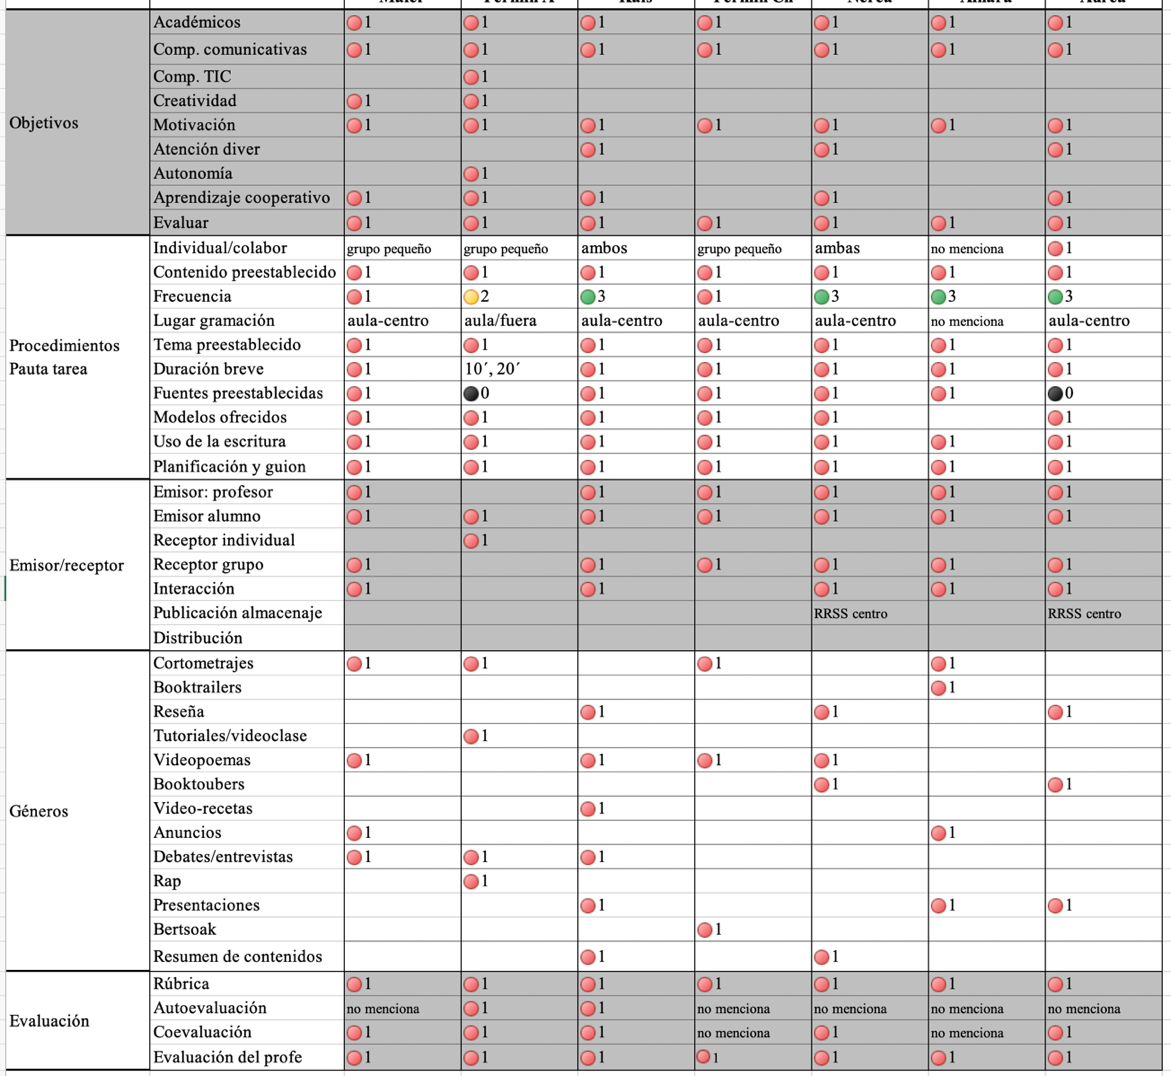
\includegraphics[width=\textwidth]{Fig3.png}
 \caption{Categorías de análisis de la base de datos (fragmento).}
 \label{fig03}
 \source{Elaboración propia.}
\end{figure}

Para analizar los vídeos construimos una lista de criterios a partir de los conceptos básicos de la grabación videográfica y de nuestra experiencia previa con vídeos discentes, la cual supervisaron dos expertos externos.

\begin{itemize}
    \item General: duración, fecha, vínculo, plataforma (YouTube, Vimeo, Instagram), autoría (firmante, titular del canal, individual/grupo/clase), nivel educativo, participación docente, público/privado, foro de reacciones (\textit{I like}, comentarios).
    \item Tema: curricular o no, literatura de adultos/infantil/juvenil, fantasía, época (antigua, medieval, renacimiento, moderna, contemporánea).
    \item Género: exposición, \textit{booktuber}, \textit{booktrailer}, técnicas específicas (\textit{draw my life}, \textit{stopmotion}, plastilina, dibujo), corto cinematográfico, clip poético (rap, videoclip), subgéneros (retos, un día con, mi casa/escuela/barrio), presentación personal.
    \item Cámara: tipo (específica, portátil, webcam, móvil con trípode), \textit{videoselfie} (cámara anterior de móvil), número (una o más).
    \item Grabación: orientación (vertical / horizontal), captura de pantalla, diapositiva con cara, respuesta ante la cámara, grabación de aula (teatro, juego de roles, entrevista, debate) o escolar (acto, extraescolar, visita), con o sin escenografía/vestuario/atrezzo.
    \item Planos: único / múltiple, estático / movimiento, con o sin cortes, ampliaciones, sin edición / edición mínima o elaborada.
    \item Voz: intradiegética (hablante visible en la imagen) / extradiegética (voz en off, externo a la imagen), voces de personajes.
    \item Grafismo: careta inicial o final, título, créditos, subtítulos (transcripción, traducción), insertados variados (iconos, \textit{stickers}), sobreimpresiones (palabras, frases).
    \item Efectos de audio: música (fondo, selectiva), sonido (pitido, campana, teléfono, silbido), silencios cortados (enunciaciones encadenadas).
    \item Efectos de imagen: filtros de color (sepia, cálido, frío), manipulación de figuras (caras, vestidos, personajes, envejecimiento), inserciones (memes, fotos, dibujos), particiones de pantalla.
\end{itemize}

Documentamos y detallamos estos procedimientos de análisis de tareas educativas de vídeo porque no hallamos bibliografía previa al respecto, dada la novedad del tema, y creemos que puede contribuir al avance en este campo.

\section{Resultados y discusión}\label{sec-formato}
Presentamos juntos los resultados del análisis de vídeos y de las entrevistas para evitar repeticiones, además de iniciar la interpretación y discusión con la investigación previa. Abordamos ocho apartados: tipos de vídeo, objetivos y contenidos, duración y frecuencia, distribución y audiencia, trabajo cooperativo, aspectos técnicos, oralidad y escritura y evaluación.

\subsection{Tipos de vídeo}\label{sec-modelo}
Identificamos estos tipos en nuestro corpus:

\begin{enumerate}
    \item \textit{Poesía/canto}: videoclips, videolits, poema musicado, rap, según los informantes, en que se recitan o cantan versos con acompañamiento visual y musical (vocal o instrumental), reciclado o creado por el propio alumno, a veces con transcripción. Ejemplo de la izquierda (\Cref{fig05}).
    \item \textit{Exposición}: resúmenes de temas curricular (autor, obra, época, estilo) con elocución discente, recreación multimodal (fotos de autores, portadas, localizaciones). Ejemplo de la derecha (\Cref{fig05})
    \item \textit{Tutoriales}: explicaciones lingüísticas/literarias (vocabulario, fraseología, puntuación, incorrecciones en canciones populares), con planteamiento instruccional y énfasis en ayudar a mejorar las destrezas y conocimientos de la audiencia.
    \item \textit{Comentarios}: paráfrasis y comentario literario de un poema o fragmento, mencionando autor, tema, contexto, interpretación y a veces con recitación.
    \item \textit{Retórica}: remix de fragmentos de canciones en que se identifican distintas figuras retóricas, con transcripción y anotación de cada figura.
    \item \textit{Periodismo}: simulaciones de géneros periodísticos como reportajes, entrevistas. Ejemplo de la izquierda (\Cref{fig06}).
    \item \textit{Cortos}: narraciones de temática diversa (juicios, thriller, misterio) simulando el cine. Ejemplo de la derecha (\Cref{fig06}).
    \item \textit{Dibujos y animación}: narración en off con apoyo gráfico (dibujos, playmóvil, viñetas de cómic, fotos) y técnicas diversas de animación (cámara lenta, stopmotion). Ejemplos con dibujos en color (izquierda), dibujos simples grabados a cámara lenta (centro) y uso de playmóvil y fotografías (derecha) para narrar (\Cref{fig07})
    \item \textit{Reseñas} (booktubers): resumen y comentario libre de lecturas, al estilo youtuber, aunque sin seguidores, I like o comentarios.
    \item \textit{Booktrailer}: vídeo promocional con estilo de thriller presentando la trama de una novela.
    \item \textit{Grabación de aula}: registro de tareas orales de clase (debates, juegos de rol), con plano general único y fijo.
    \item \textit{Presentaciones}: de alumnos (videocurrículums, intereses), centros y ciudades (para intercambios).
\end{enumerate}

\begin{figure}[htbp]
 \centering
 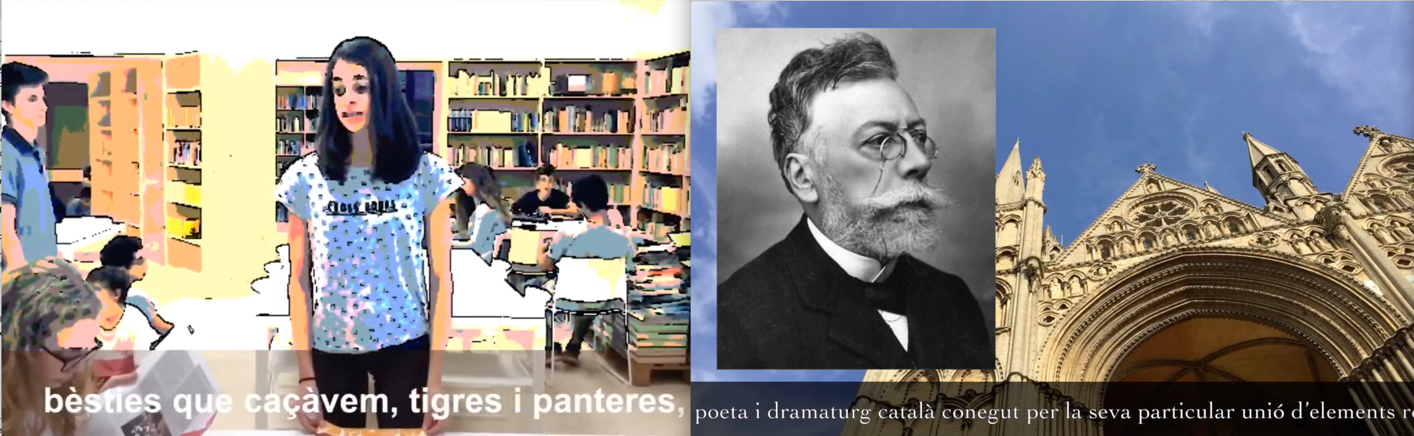
\includegraphics[width=0.85\textwidth]{Fig6.png}
 \caption{Captura del videopoema de Guilgamesh (4º ESO, izquierda) y exposición sobre La Renaixença (1º BACH, derecha), del Colegio Sant Miquel dels Sants), de las clases de literatura de 2019 de Sílvia Caballeria (blog Què us diré?).}
 \label{fig05}
 \source{Elaboración propia.}
\end{figure}

\begin{figure}[htbp]
 \centering
 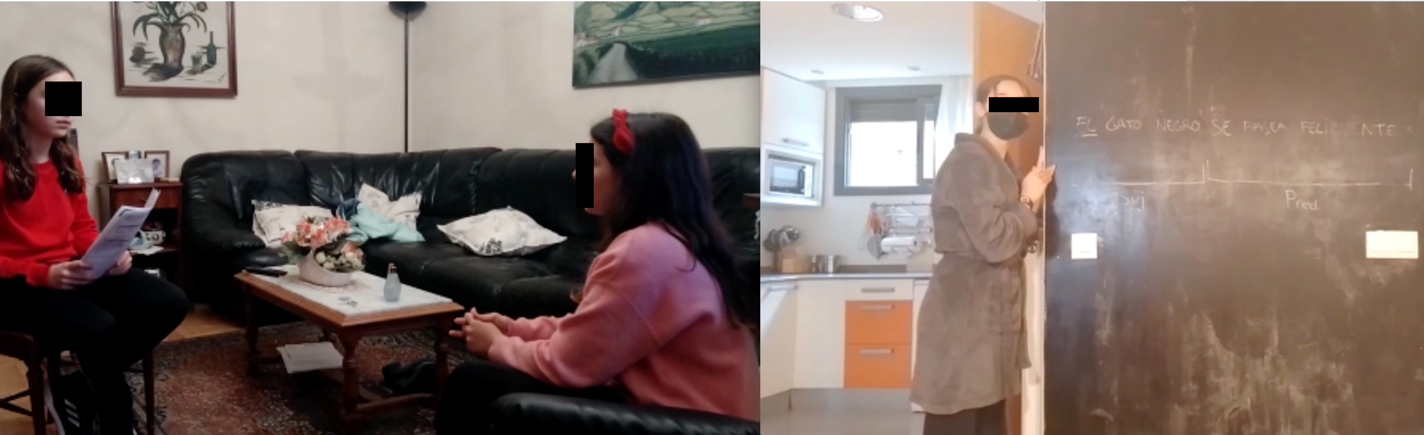
\includegraphics[width=0.85\textwidth]{Fig7.png}
 \caption{Captura de entrevista a Garcilaso de la Vega (izquierda) y corto parodiando una clase de sintaxis (derecha), de las clases de Lengua y literatura castellana de Fermín Areta en el BHI Eunate (1º ESO, 2021).}
 \label{fig06}
 \source{Elaboración propia.}
\end{figure}

\begin{figure}[htbp]
 \centering
 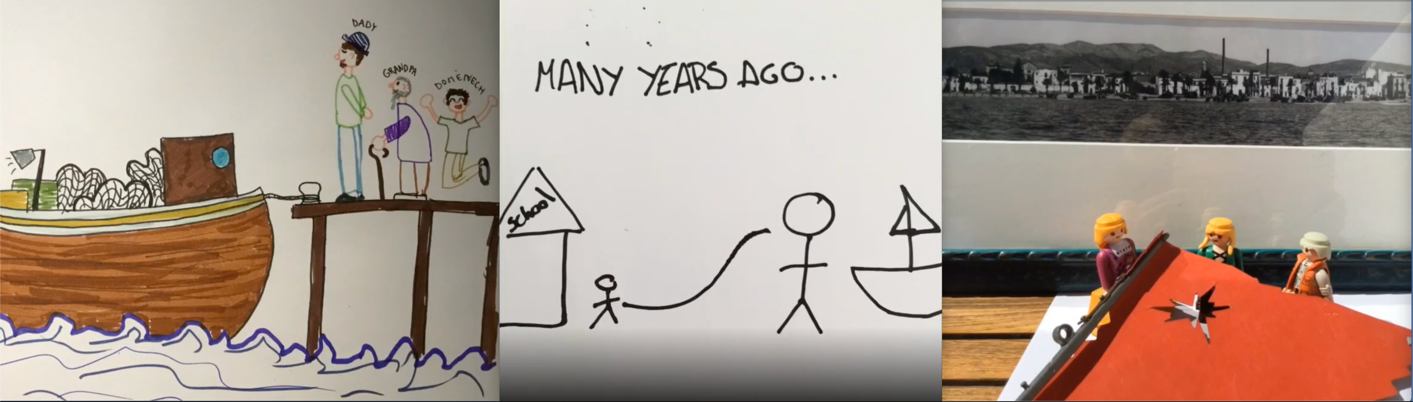
\includegraphics[width=0.85\textwidth]{Fig8.png}
 \caption{Capturas de vídeos de dibujos y animación recordando la actividad pesquera de los abuelos del alumnado de 30 de ESO (IES Baix a mar, Vilanova i la Geltrú, 2021), en las clases de inglés de Anna Brull.}
 \label{fig07}
 \source{Elaboración propia.}
\end{figure}

Hallamos varios ejemplos de la gran mayoría de estos tipos en nuestro corpus, a menudo de procedencia diversa, por lo que consideramos esta relación como una tipología empírica provisional. No hemos cuantificado la frecuencia de cada tipo porque con un corpus intencional los datos carecerían de valor estadístico y porque algunos vídeos pueden compartir rasgos de dos o más tipos.

Un aspecto final de la mayoría de vídeos que conviene destacar es su carácter lúdico, a veces más explícito (parodias, juegos humorísticos, recursos divertidos) a veces menos (actitud divertida del alumnado). Un ejemplo de ello es un corto de los alumnos de Areta que simulan en una cocina una clase de sintaxis, con pizarra, explicación, preguntas, correcciones y un alumno dormido (\Cref{fig06}, derecha).

Las entrevistas confirman esta tipología, aunque los docentes no siempre usen los mismos términos. Así, pueden referirse a debates (grabados en el aula) o entrevistas y anuncios (géneros periodísticos), a resúmenes de contenido (exposiciones) o a recetas (tutoriales). Una categoría con mucha diversidad terminológica es la videopoesía, que engloba la versificación (\textit{bertsoak} [eusquera] con tradición propia, rap o hip-hop en inglés y otros idiomas), la recitación y el canto o la animación de grabaciones de terceros.

Entrando en la discusión, algunos de estos tipos son géneros socialmente establecidos, con rasgos definidos y cierta popularidad como la videopoesía \cite{aliagas_rapping_2016}, los mencionados \textit{booktubers} y \textit{booktrailers}, el periodismo o los cortos. Otros tienen cierta tradición como recursos para aprender idiomas, como las presentaciones personales y los dibujos y la animación \cite{shafirova_identity_2020}.

En cambio, hallamos categorías más inestables, divergentes o menos preestablecidas, como la grabación de aula, que incluye intenciones y temas diversos, o los tutoriales, que presentan una gran diversidad interna. En el proyecto \textit{Ensenyem la llengua} de Godoy (Tabla 1), los estudiantes crean “tutoriales para enseñar lengua”, con resultados variados y creativos, como un concurso onomasiológico de vocabulario, que remite al reto \textit{youtuber}, o unos buscadores de errores en Twitter que metaforizan su tarea con imágenes de cazadores de pájaros en un bosque, parodiando un popular programa televisivo sobre buscadores de setas (\textit{Caçadors de bolets}, TV3).

La paulatina digitalización abre otra perspectiva de análisis, puesto que algunos tipos (poesía, exposición, comentario, retórica, periodismo) remiten a prácticas didácticas analógicas como la lectura poética, la monografía sobre un autor u obra, el comentario de texto, el catálogo de figuras retóricas o la redacción de noticias. En este caso, el paso de la escritura al vídeo multiplica las posibilidades expresivas del alumnado, que en la red accede a material multimedia más atractivo (cine, música, imagen), fuentes diversas y formatos más cercanos. Dos ejemplos de este salto cualitativo son un videopoema de gran calidad de una alumna de García sobre “Cuando lloro” de Fran Alonso, con fotografías propias en blanco y negro y música de fondo de Satie (\textit{Gymnopédies}), o el \textit{Homenaje a Gloria Fuertes} citado en Metodología y corpus.

Por otra parte, algunos tipos (\textit{tutoriales, booktubers, booktrailers}) son posteriores a la red, se alimentan de la popularidad adquirida en las redes sociales y el alumnado los copia o simula con poca variación. Tipos menos afiliados se benefician también del acceso a modelos y ejemplos (\textit{presentaciones}) o al material musical y poético (\textit{retórica}) para hallar contenido para sus obras.


\subsection{Objetivos y contenidos}\label{sec-organizacao}
Los once docentes coinciden en que la grabación de vídeos es una tarea formal y evaluable de la materia, con objetivos y contenidos curriculares preestablecidos. Para muchos es “la tarea final”. Reconocen también su valor motivacional y el incremento y la mejora de la competencia lingüística/literaria que supone, pero coinciden menos en su valor para atender a la diversidad, fomentar la creatividad o mejorar la competencia digital o la autonomía del aprendiz. (Aclaremos que atender la diversidad es muy relevante para varios de los entrevistados, con alumnado migrado, con fracaso escolar o discapacidad).

En su práctica docente, Caballeria (autora del blog “Què us diré?” desde 2008, con 628 entradas y decenas de recursos) fija la obra literaria (contenido) que trabajará su alumnado, los plazos de entrega y los procedimientos mínimos (lectura y comprensión de la obra, redacción del \textit{storyboard}, uso de transcripción escrita) del producto final, que son los objetivos didácticos e incluyen los criterios de evaluación. Luego, en este marco, sus alumnos eligen un tema específico de la obra (personaje, capítulo, aspecto) y unas técnicas o formatos de su gusto. Así, uno hace 3D, animación, realidad aumentada, composición y canto, pero “facin el que facin […] cada cop més el producte final es un vídeo.” De modo que el vídeo permite integrar el resto de técnicas o recursos que interesan al estudiante y facilita que este se pueda apropiar de la tarea literaria. En esta línea, Bayano fija el vocabulario específico y los conectores que deben usar sus bachilleres en eusquera (nivel C1) al parodiar un episodio del popular \textit{reality} de la televisión vasca (\textit{Baserria}).

En su proyecto sobre la comedia nacional de Lope de Vega, Areta propone a su alumnado de 3º de ESO grabar fragmentos de teatro para “encontrar los arquetipos de los personajes lopescos y después intentar actualizarlos, hacer una especie de comedia nacional del siglo XXI, […] en una discoteca o en un instituto, siendo el galán enamorado un chico de clase, siendo el gracioso el graciosillo de clase”. Al grabar una entrevista distendida a Garcilaso (\Cref{fig07}, izquierda), simulando los programas de televisión, espera que el alumnado pregunte sobre “su vida privada, sobre asuntos que le gustaba tratar en su poesía […], así para eso antes se veía documentación previa, [los alumnos] tienen que saber quién era Garcilaso y cuáles son las características de su poesía y luego podían construir la entrevista”.

Entrando en la discusión, estos ejemplos muestran que el uso del vídeo acerca los contenidos literarios antiguos al día a día del alumnado, porque el cambio de formato implica forzosamente una adaptación del contenido. En este sentido, la investigación previa sugiere que la producción de vídeo incrementa la autonomía del aprendiz \cite{vasquez_bustamante_aprendizaje_2013,oechsler_mathematical_2020} y su creatividad \cite{yeh_exploring_2018}, aunque los docentes no lo destaquen.

\subsection{Duración y frecuencia}\label{sec-organizacao-latex}
Se graban pocos vídeos y son más breves que largos. La frecuencia va de uno a tres por trimestre, aunque haya periodos sin actividad. Según el género, la mayoría de vídeos es breve (1-2’), con algunas producciones más largas (sobre 3-6’) y pocas excepciones (más de 8’). Videopoesía, presentaciones y dibujos y animaciones duran menos de 2’; reseñas (booktubers), tutoriales y periodismo, 3’-5’; las exposiciones monográficas y los cortos, algo más (5’-7’); solo la grabación continuada de aula (debates) o alguna exposición académica superan la decena de minutos, pero podemos hallar varias excepciones a estos parámetros. Para Chivite: “mejor que no sean demasiado cortos, porque no merece la pena montar todo el aparataje para eso”.

Pero pese a la brevedad y relativa frecuencia, estas tareas ocupan mucho tiempo, porque “primero necesitan analizar vídeos reales; después un ejemplo de cómo se hace, y después ya lo hacen ellos” (Chivite). En la misma línea, Areta distingue las siguientes fases en un proyecto de grabación: la documentación (búsqueda de fuentes) en que docente y alumno negocian las fuentes de información; la programación en que el alumnado escribe los guiones a partir de la información anterior; la grabación en las localizaciones elegidas, con la caracterización necesaria; la edición final y su pase o compartición con el grupo. Se trata, entonces, de un proyecto ambicioso que puede ocupar varias semanas y que exige también trabajo fuera del aula, en varias fases (grabación, documentación). Por ello el número de proyectos suele ser bajo.

Estos datos coinciden con \textcite{nikitina_video-making_2010}, para la que los vídeos breves presentan menos dificultades técnicas, se integran mejor en un calendario apretado de clases con un programa de asignatura muy cargado.

\subsection{Distribución y audiencia}\label{sec-titulo}
La mayoría de docentes distribuye los vídeos en la plataforma cerrada de clase (Classroom, Moodle), aunque la mitad (\Cref{tab01}: Brull, Caballeria, Godoy, Ouelhazi, Ugalde) publica en abierto una selección de obras, en espacios personales (YouTube, Blogspot, Wevideo, padlet) o institucionales (centro, eTwinning), que actúa como acicate y motivación para futuras promociones. Algunos estudiantes publican sus vídeos en su canal personal (YouTube), aunque carezcan de seguidores y comentarios. Algún docente afirma tener un espacio de pago, pero la mayoría utiliza el servicio gratuito, con limitaciones en duración y número de publicaciones. Algunos docentes publican también vídeos personales, vinculados con su docencia.

Según las entrevistas, muchos docentes dedican tiempo a visualizar los vídeos en clase, en línea o en tutorías, a comentarlos informalmente e incluso a coevaluarlos con rúbricas (ver Sección \ref{sec-secoes}), de modo que se desarrolla un ciclo comunicativo completo, aunque sea dentro del recinto escolar. Algunos ceden la decisión de mostrarlos o no a cada grupo, con resultados variados. Areta sugiere que los aprendices más trabajadores con mejores productos tienen más ganas de mostrarlo a sus compañeros que vergüenza, y cita ejemplos de alumnos “frikies” que merecieron el aplauso de su clase por su vídeo. Sin duda, el carácter público o privado del vídeo regula su audiencia real y tiene notable influencia en la predisposición del alumnado hacia la tarea.

Estos resultados coinciden con nuestra encuesta al profesorado de secundaria \cite{cassany_ya_2021}, en que docentes y alumnado muestran inseguridad respecto a estas cuestiones éticas y de privacidad, hasta el punto de que solo un 11\% publica vídeos en abierto, pese al potencial didáctico que posee la publicación del vídeo en abierto con la posibilidad de recibir comentarios reales, de poder responderlos y de practicar la escritura.

\subsection{Trabajo cooperativo}\label{sec-autores}
En nuestro corpus abundan los vídeos de pareja y pequeño grupo en distintas modalidades, en los que los coautores se reparten minutos y protagonismo o bien se distribuyen las tareas detrás de la cámara, según indican los créditos. La gran mayoría de vídeos de grupos completos (15 o más aprendices) son grabaciones de aula, con alguna excepción, como la recitación en grupo (un verso por alumno) del \textit{Lamento de Enkidu} (Guilgamesh) en la biblioteca del centro, con filtros de imagen y un plano único con travelling al estilo \textit{lip dub} (\Cref{fig05}, izquierda, con alumnos de Caballeria).

Las entrevistas confirman que las grabaciones se hacen en pequeños grupos o tanto en grupo como individualmente, y que la cooperación entre alumnos motiva a los más tímidos a superarse para no perjudicar a sus compañeros. Areta se presenta ante su alumnado como Netflix (“yo soy Netflix y me gustaría tener un programa de esto”) y firma un contrato con cada grupo, “con DNI”, que especifica las condiciones del trabajo en equipo: “se trabaja tanto dentro como fuera del aula”, “tienes que quedarte 3 semanas por las tardes” o quien “no está trabajando lo suficiente […]” lo puede expulsar un grupo y tendrá que hacer los vídeos individualmente”.

Los vídeos individuales son minoritarios, breves, más sencillos técnicamente y suelen responder a tareas verbales concretas de clase, como las presentaciones, la videopoesía y los booktubers, aunque haya varias excepciones. La literatura previa confirma de manera generalizada que la grabación de vídeos fomenta la cooperación entre el alumnado (apartado 2) e, indirectamente, incrementa la centralidad del aprendiz en el aula y su autonomía \cite{vasquez_bustamante_aprendizaje_2013}.

\subsection{Aspectos técnicos}\label{sec-idioma}
En la parte técnica, hallamos gran diversidad de formatos, recursos y estilos. Los vídeos más simples son breves, utilizan un plano único fijo, carecen de edición (créditos, cortes, música), parecen ser producto de una estrategia básica de “ensayo, error y repetición”, buscando una grabación aceptable, y actúan como respuestas verbales ante la cámara o grabaciones de actividad de aula. Los vídeos individuales se asocian más con este modelo.

En cambio, los vídeos más complejos delatan más planificación, ediciones sofisticadas de imagen y sonido, con planos variados, juegos de imagen (B/N, cámara lenta, filtros de color y contorno), inserción de ítems visuales (fotos, dibujos, esquemas) o auditivos (música, aplausos, pitidos, etc.), recorte de silencios para ganar rapidez o subtitulación gráfica (transcripción, traducción a otros idiomas). Muchos de estos efectos técnicos provienen de la experticia que el alumnado ha obtenido participando en las redes sociales de vídeo (Instagram, TikTok) fuera del centro. Estos vídeos suelen ser obra de grupos que se distribuyen las tareas y suman las habilidades de cada miembro.

Los vídeos se graban en el entorno (centro, domicilio, barrio, parque), aprovechan recursos propios (vestuario, atrezzo, juguetes) e incorporan efectos visuales (tomas falsas, carta de ajuste, iconos de Netflix o 20th Century Fox), acústicos (sintonías, aplausos) o gráficos (tipografías populares, expresiones en inglés [\textit{the end, bye}]) con finalidades paródicas.


\subsection{Oralidad y escritura}\label{sec-resumo}
Las destrezas orales y escritas desempeñan funciones importantes y variadas en la grabación de vídeos. Veamos primero sus roles en el producto final del vídeo y a continuación sus roles en la tarea completa de grabación.

Respecto al habla, hallamos monólogos informales y aparentemente espontáneos en las respuestas breves ante la cámara o en intervenciones de clases grabadas. Pero lo más habitual son elocuciones relativamente fluidas, cercanas al teatro o al cine, con un registro más coloquial, o exposiciones periodísticas y académicas con un grado de formalidad más alto y el uso de ciertos términos de la disciplina. Estas producciones sugieren la existencia de un trabajo previo de elaboración, ensayo y memorización de estos discursos que probablemente utilice un modo específico de escritura, que es la de redactar para oralizar y grabar lo que la audiencia va a escuchar sin poder leer. En el corpus el alumnado ejecuta aceptablemente su parte, sin dudar ni tropezar ni consultar los apuntes y dirigiendo la mirada hacia el interlocutor adecuado.

En cambio, la escritura asume comparativamente roles secundarios como la anotación sobreimpresa (créditos, localizaciones y fechas históricas, citas, aclaraciones), la inserción de elementos gráficos (capturas de WhatsApp, carteles) o la grabación natural de escritos (carteles, pizarras, portátiles o papeles), como la técnica youtuber (draw my life) de grabar la mano que escribe/dibuja sobre papel blanco mientras el habla en off comenta el contenido. Finalmente, solo el alumnado de Caballeria incorpora la transcripción de manera sistemática en sus vídeos, de modo que ofrece su texto tanto hablado como en subtítulos rápidos, claros y correctos (ver \Cref{fig05}).

Todos los docentes reconocen que el alumnado realiza algún tipo de escritura para preparar la grabación y que este se valora: “Hay un trabajo escrito que se valora más que el vídeo incluso” (Chivite); “hacemos una especie de boceto […] que suelo corregir […] les pido que no se puede leer, sí que pueden usar una chuletilla para construir el texto oral” (Bayano)”. Dos docentes aportan ejemplos al respecto.

En su proyecto Los expresionistas, de lengua castellana, Not propone grabar vídeo sin habla para analizar la conducta no verbal, para lo cual los bachilleres debían redactar un guion con presentación del vídeo propuesto, relación de escenas y su descripción, reflexión sobre el contenido y aportación personal. Los 11 guiones aportados son escritos grupales de 200-500 palabras con lenguaje general que describen los vídeos. En la misma línea, Caballeria crea una plantilla en Excel que su alumnado completa (\Cref{fig08}) y entrega a la docente antes de la grabación.

\begin{figure}[htbp]
 \centering
 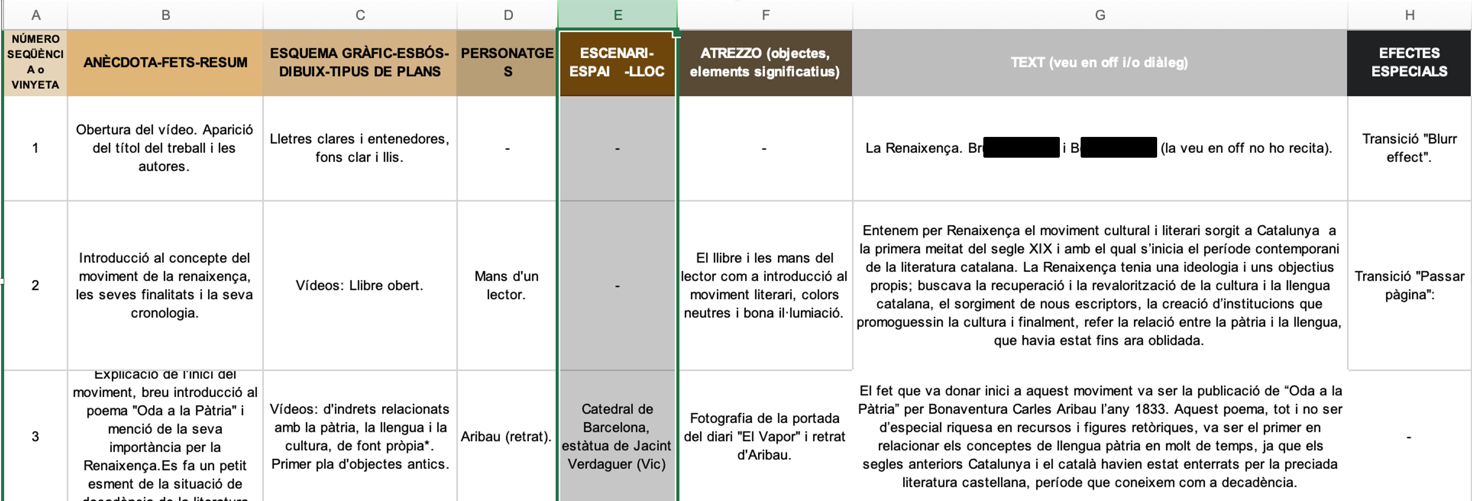
\includegraphics[width=\textwidth]{Fig5.png}
 \caption{Plantilla de storyboard (del blog Què us diré?) de dos bachilleres para una exposición académica sobre literatura catalana del siglo XIX.}
 \label{fig08}
 \source{Elaboración propia.}
\end{figure}

Nuestros resultados coinciden en muchos puntos con trabajos previos. \textcite{cassany_ya_2021} hallaron que más del 90\% de los docentes de secundaria encuestados usaba la escritura previa para planificar una grabación, pero solo un 7,6\% afirmaba usar la subtitulación en la edición del vídeo, pese a los trabajos que reconocen su alto potencial didáctico para los idiomas \cite{cassany_daniel_coord._fandom_2019} o al proyecto europeo \hyperlink{http://clipflair.net/}{Clipflair}.

\subsection{Evaluación}\label{sec-secoes}
Todos los docentes coinciden en usar rúbricas propias para evaluar la grabación, aunque de diversa manera: 6 incluyen porcentajes de coevaluación y 2 de autoevaluación, en varios porcentajes. A modo de ejemplo, Areta detalla la evaluación de los cuatro vídeos que hizo su alumnado en 2020-21 (ejemplos de la \Cref{fig06}):

\begin{quote}
    Le reservo un 20\% a la heteroevaluación (del docente a los alumnos) [basada en la observación del trabajo diario del alumno]; después reservo un 10\% para la coevaluación (con una rúbrica evalúan al resto del grupo); después, una autovaluación [otro 10\%] (con la misma rúbrica evalúan su propio trabajo). Ese 40\% es la nota [del trabajo de cada alumno]. El otro 60\% serían cuatro productos [vídeos], cada uno son el 15\%; un 5\% para el guion, un 10\% para lo que es el vídeo en sí. Tanto el guion como el vídeo tienen una rúbrica: el guion tiene que ver más con la corrección ortográfica y tipográfica, y el vídeo con el contenido tanto audiovisual como verbal [porque] es importante cómo hablan, no solo qué hablan. (Entrevista a Fermín Areta).
\end{quote}

Las rúbricas son relativamente simples, emplean un lenguaje general e incorporan iconos populares, para que el alumnado los pueda utilizar sin dudas. Not aporta este ejemplo (\Cref{fig09}) del mencionado proyecto Los expresionistas.

\begin{figure}[htbp]
 \centering
 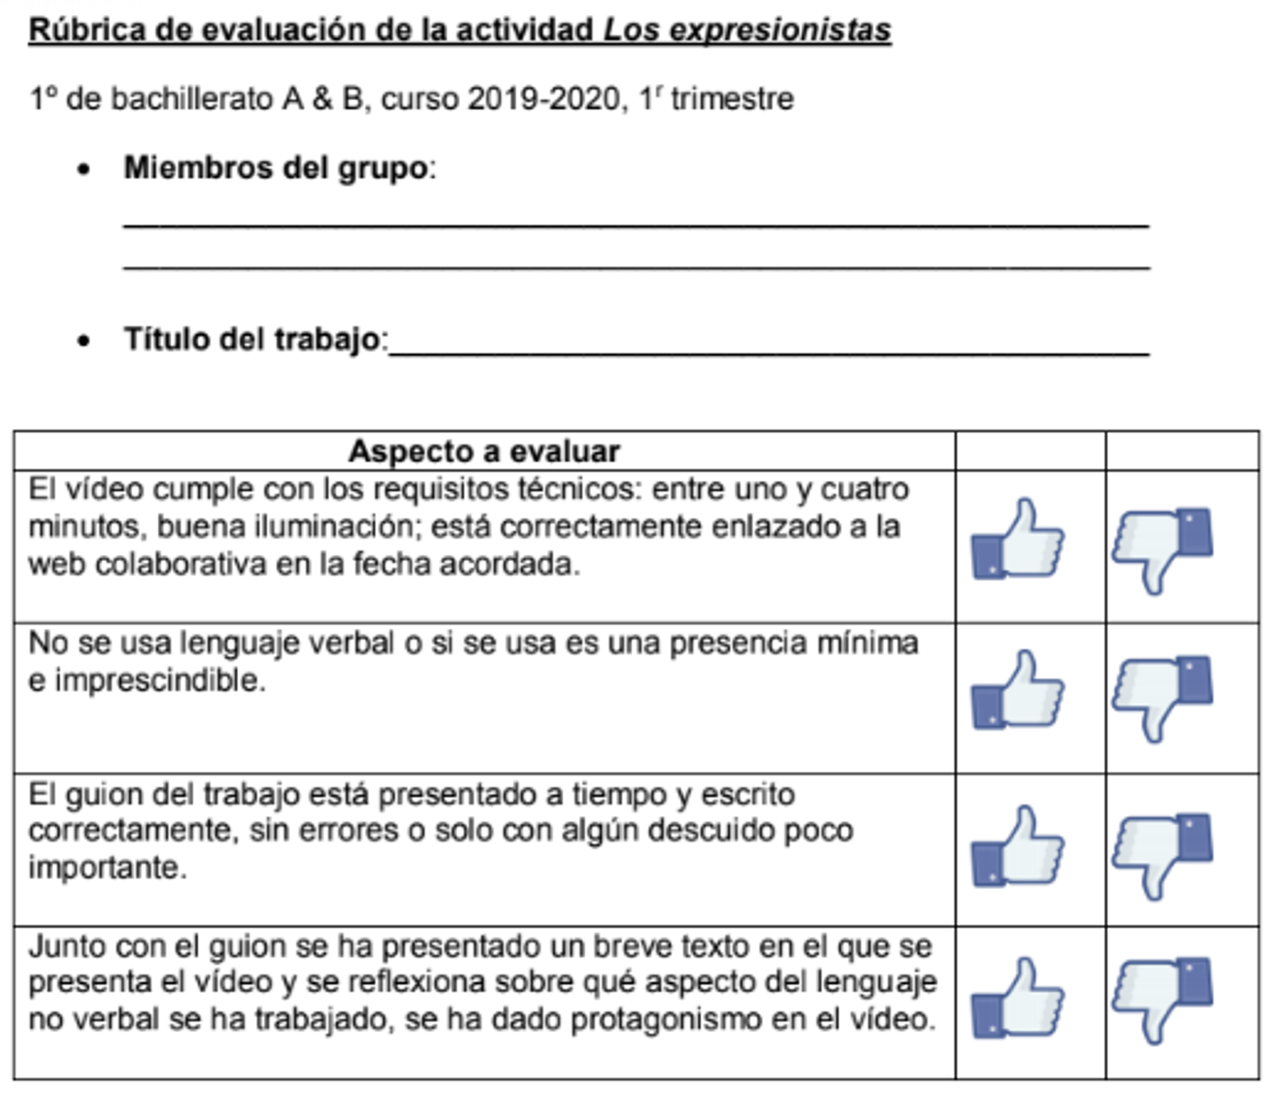
\includegraphics[width=0.85\textwidth]{Fig10.png}
 \caption{Rúbrica de evaluación (Anton Not, INS La Serra, Mollerussa).}
 \label{fig09}
 \source{Elaboración propia.}
\end{figure}

\section{Conclusiones}\label{sec-format-simple}
Respondemos a nuestras preguntas de investigación. Respecto a la primera, hemos identificado 12 tipos de vídeos, que muestran su versatilidad y riqueza, además de describir las buenas prácticas realizadas con la voz de sus docentes expertos. Esta tipología amplía notablemente los videogéneros descritos en la investigación previa (apartado 2).

Sobre la cuestión de qué aprendizajes literarios promueven, concluimos que los vídeos abordan un abanico amplio de contenidos, con aproximaciones más historicistas (exposiciones sobre literatura antigua/medieval/renacentista, etc.), o más competenciales, sean receptivas (\textit{booktubers}, comentario) o productivas (recitación, narración, presentación). Otro punto relevante es que el formato audiovisual permite relacionar más fácilmente el currículum literario con las enseñanzas artísticas y con las diversas lenguas del centro.
Además, nuestro análisis permite identificar las 18 actividades verbales implicadas en la elaboración de vídeos discentes (ver \Cref{tbl2}), que abarcan la comprensión y la producción oral y escrita en las etapas principales de planificación, grabación, edición y recepción.

\begin{table}[htbp]
\caption{Tareas verbales que desarrolla el alumnado al grabar vídeos.}
\label{tbl2}
\centering \small
\begin{tabular}{p{2cm} p{12cm}}
\toprule
Planificación & 1 Comprender y valorar las consignas de las tareas y los modelos aportados.

    2 Redactar un proyecto (\textit{storyboard}): planos, ambientación, actores, imagen, efectos.
    
    3 Documentarse y elegir el contenido del vídeo: conceptos, argumento, situaciones.
    
    4 Documentarse y seleccionar material visual (imágenes, grafismo) y auditivo (música, efectos).
    
    5 Cumplir las normas éticas (respeto, privacidad, citación) de las fuentes usadas.
    
    6 Redactar el guion completo del vídeo con el texto de todos los personajes y voces. \\ 
\midrule
Grabación     & 7 Gestionar la actividad del grupo durante la grabación, razonando y dando instrucciones.

    8 Preparar, memorizar y ensayar el guion: poemas, elocución, diálogos.
    
    9 Actuar ante la cámara integrando la enunciación oral con el resto de aspectos no verbales.
    
    10 Visualizar (escuchar y valorar) la grabación realizada y valorar su calidad.  \\ 
\midrule
Edición &     11 Editar la imagen y el audio del vídeo con las grabaciones y el material previo elegido.

    12 Decidir, recoger, redactar e insertar los créditos completos del vídeo.
    
    13 Transcribir la enunciación oral con subtítulos e insertarlos en el vídeo.
    
    14 Traducir la enunciación o su transcripción a otro idioma e insertarlo en el vídeo. \\
\midrule
Recepción &     15 Publicar el vídeo final en la plataforma e informar a la audiencia.

    16 Presentar el vídeo a su audiencia (docente, clase, centro), en línea o cara a cara.
    
    17 Seguir, valorar y replicar a los comentarios de la audiencia.
    
    18 Evaluar con los coautores y el docente las reacciones de la audiencia. \\
\bottomrule
\end{tabular}
\source{Elaboración propia.}
\end{table}

Sin duda, dependiendo del tipo de vídeo grabado y del diseño didáctico de la práctica se desarrollarán unas u otras de estas actividades verbales.

Respecto a la segunda pregunta, detallamos las tres potencialidades y limitaciones más relevantes. Entre las primeras:

\begin{itemize}
    \item \textit{Agencia del aprendiz}. La grabación en vídeo relaciona el currículum con la cultura audiovisual del aprendiz (series, música, televisión) o “unifica el mundo académico con su realidad extraescolar [del alumnado]” (Areta), porque “los veo [los alumnos] más sueltos grabando un vídeo que escribiendo; [...] al vídeo sí le ven salida; si escribimos algo, al final no lo van a enseñar a nadie [...]” (Chivite). Por ello, esta tarea ofrece las condiciones idóneas para desarrollar la agencia del aprendiz \cite{biesta_agency_2007}: para que pueda regular su actividad, aportar su voz al vídeo, tomar conciencia y asumir responsabilidades. Nuestro análisis aporta numerosos ejemplos de este hecho, en los vídeos que incluyen conocimientos y destrezas que no forman parte del currículum, como las parodias de programas populares de televisión o los estilos youtuber (\textit{lip dub, draw my life}) \cite{ogrady_developing_2022}.
    \item \textit{Ciclo comunicativo}. A diferencia de la escritura, el vídeo facilita la conexión con una audiencia real para desarrollar ciclos comunicativos completos, con reacciones (\textit{I like}), comentarios y réplicas. Un vídeo privado para el docente es una tarea escolar parecida a una redacción o un examen, pero un vídeo público comunica con audiencias externas al centro, creando contextos nuevos y motivadores para al alumnado. Esta opción todavía tiene más valor en una materia artística como la literatura, en la que el alumnado vuelca sus sensibilidades. Como reconoce Garde: “fue muy interesante la reacción de las familias al ver a sus hijos trabajando”. Este punto coincide con la práctica booktuber fuera del aula de reaccionar a los vídeos \cite{fialho_booktubers_2023,tomasena_glennie_booktubers_2020}.
    \item \textit{Motivación}: Aunque no sea la primera ventaja destacada, la motivación que aporta la grabación de vídeos tiene efectividad: [El vídeo es] “un dopaje total”, sugiere Garde, tanto para el alumnado como para el docente: “¡Qué provecho le sacamos! A los chavales les gusta. Aunque les da vergüenza, les gusta. […] Lo audiovisual es una entrada directa a nuestros alumnos” (Garde); es “esa manera de relacionarse emocionalmente” con el currículo (Bayano).
\end{itemize}

Veamos ahora algunas limitaciones:

\begin{itemize}
    \item \textit{Adaptación al alumno}. Algunos grupos no responden a las expectativas por su actitud o falta de trabajo, de modo que la grabación fracasa u obtiene resultados pobres. Para Chivite “hay que saber leerlos”, refiriéndose a los alumnos, a descubrir si poseen la actitud y el “ritmo y deseo de trabajo” necesarios para hacer este tipo de tareas; este docente dedica la primera evaluación a diagnosticar al grupo y, si va bien, propone la grabación de vídeos para la segunda evaluación. Del mismo modo, Caballeria hace una encuesta previa de intereses con la petición de formular tres deseos priorizados del vídeo que se quiere hacer, para decidir temas, hacer grupos y buscar el mejor proyecto.
    \item \textit{Cuestiones éticas}. Muchos docentes dudan y muestran inseguridad con las cuestiones éticas de privacidad, derechos del menor, publicación en abierto de vídeos, derechos de autor, etc. Así, Ugalde reconoce que: “no conviene sacar imágenes del alumnado, intentamos hacer vídeos en los que aparezcan muñecos [dibujos, fotos, etc.]; hay que buscar formas indirectas” para mantener la privacidad del menor. Sin duda, ofrecer modelos de consentimiento informado, repositorios de música, imágenes e iconos libres de derechos o repositorios institucionales protegidos, podría facilitar la grabación de vídeos del alumnado.
    \item \textit{Formación tecnológica}. No todos los entrevistados se sienten seguros con su dominio de la tecnología. Garde confiesa que “he aprendido a hacer vídeos, que no tenía ni idea” al participar en un proyecto eTwinning y colaborar con otros centros. Muchos también reconocen que han aprendido por su cuenta, más solos que en programas oficiales, por lo que la formación de profesorado aquí evidencia también objetivos que cumplir.
\end{itemize}

Este trabajo cuenta con algunas limitaciones, como un número reducido de informantes y vídeos, sin representatividad del amplio y diverso campo de la secundaria educativa. Tampoco hemos podido acceder al punto de vista del alumnado, el principal protagonista, que queda para trabajos futuros. Finalmente, otro formato verbal que esperamos poder estudiar en el futuro es el podcast o las grabaciones de audio, que mantienen muchas de las potencialidades del vídeo sin alguno de sus inconvenientes.

\section{Financiación}\label{sec-conclusao}
Este trabajo forma parte del proyecto El vídeo como formato de aprendizaje dentro y fuera del instituto (\hyperlink{https://sites.google.com/view/forvid/home}{ForVid}) financiado por el Ministerio de Ciencia e Innovación (RT2018-100790-B-100). También ha aprovechado fondos del grupo competitivo GRAEL procedentes del gobierno catalán (AGAUR, 2017SGR 915). Agradecemos a todos los participantes en el proyecto (docentes, autoridades de centros, técnicos de investigación) su tiempo y dedicación al mismo; también agradecemos a Liudmila Shafirova y Marc Urrutia, técnicos de investigación, su ayuda para recopilar datos del corpus y procesarlos.


\printbibliography\label{sec-bib}
% if the text is not in Portuguese, it might be necessary to use the code below instead to print the correct ABNT abbreviations [s.n.], [s.l.]
%\begin{portuguese}
%\printbibliography[title={Bibliography}]
%\end{portuguese}


%full list: conceptualization,datacuration,formalanalysis,funding,investigation,methodology,projadm,resources,software,supervision,validation,visualization,writing,review
\begin{contributors}[sec-contributors]
\authorcontribution{Consuelo Allué}[datacuration,investigation,methodology,resources,validation,visualization,writing,review]
\authorcontribution{Daniel Cassany}[conceptualization,methodology,investigation,projadm,supervision,visualization,writing,review]
\end{contributors}



\end{document}

